% =====================================================================
%  HATI -- Status & Roadmap report (for external scientific review)
%  Author: Gergő Csaba Morvai
%  Engine: LuaLaTeX  (compile: latexmk -lualatex hati_status_roadmap.tex)
% =====================================================================
\documentclass[11pt]{article}

\usepackage{fontspec}
\usepackage{microtype}
\usepackage[a4paper,margin=2.45cm]{geometry}
\usepackage{graphicx}
\graphicspath{{../output/athena/}{../output/}}
\usepackage{amsmath,amssymb}
\usepackage{xcolor}
\usepackage{booktabs}
\usepackage{array}
\usepackage{siunitx}
\usepackage[font=small]{caption}
\usepackage{enumitem}
\usepackage{tcolorbox}
\tcbuselibrary{skins,breakable}
\usepackage{titlesec}
\usepackage[backend=biber,style=authoryear,sorting=nyt,maxcitenames=2,uniquelist=false]{biblatex}
\addbibresource{references.bib}
\usepackage[hidelinks]{hyperref}
\usepackage{cleveref}

\setmainfont{TeX Gyre Pagella}
\setsansfont{TeX Gyre Heros}[Scale=0.92]
\setmonofont{TeX Gyre Cursor}[Scale=0.90]

\definecolor{hatiblue}{HTML}{1F3A5F}
\definecolor{hatiaccent}{HTML}{B23A2E}
\definecolor{hatiteal}{HTML}{1B7A6E}
\definecolor{plainbg}{HTML}{EAF2FB}
\definecolor{plainframe}{HTML}{2E6DB4}
\definecolor{intentbg}{HTML}{F0EEF6}
\definecolor{intentframe}{HTML}{5B4B8A}
\definecolor{limitbg}{HTML}{FBEEEC}
\definecolor{limitframe}{HTML}{B23A2E}
\definecolor{okbg}{HTML}{EAF5EF}

\titleformat{\section}{\sffamily\Large\bfseries\color{hatiblue}}{\thesection}{0.6em}{}
\titleformat{\subsection}{\sffamily\large\bfseries\color{hatiblue!88}}{\thesubsection}{0.5em}{}
\titlespacing*{\section}{0pt}{1.6ex plus .3ex}{0.8ex}

\newtcolorbox{plainbox}{breakable,enhanced,colback=plainbg,colframe=plainframe,
  boxrule=0.6pt,arc=2pt,left=7pt,right=7pt,top=4pt,bottom=4pt,
  fonttitle=\bfseries\sffamily\small,coltitle=plainframe,
  attach boxed title to top left={xshift=8pt,yshift=-7pt},
  boxed title style={colback=plainbg,colframe=plainframe,boxrule=0.4pt,arc=1pt},title={In plain words}}
\newtcolorbox{intentbox}{breakable,enhanced,colback=intentbg,colframe=intentframe,
  boxrule=0.6pt,arc=2pt,left=7pt,right=7pt,top=4pt,bottom=4pt,
  fonttitle=\bfseries\sffamily\small,coltitle=intentframe,
  attach boxed title to top left={xshift=8pt,yshift=-7pt},
  boxed title style={colback=intentbg,colframe=intentframe,boxrule=0.4pt,arc=1pt},title={Why it is built this way}}
\newtcolorbox{limitbox}{breakable,enhanced,colback=limitbg,colframe=limitframe,
  boxrule=0.6pt,arc=2pt,left=7pt,right=7pt,top=4pt,bottom=4pt,
  fonttitle=\bfseries\sffamily\small,coltitle=limitframe,
  attach boxed title to top left={xshift=8pt,yshift=-7pt},
  boxed title style={colback=limitbg,colframe=limitframe,boxrule=0.4pt,arc=1pt},title={Honest limit}}

\sisetup{detect-all,per-mode=symbol}
\DeclareSIUnit{\px}{px}
\setlist{nosep,leftmargin=1.4em}
\captionsetup{labelfont={bf,sf,color=hatiblue}}

\title{\sffamily\bfseries\color{hatiblue}\LARGE HATI: Current State and Forward Plan\\[3pt]
\Large\mdseries A status and roadmap report on a physics-based, two-channel\\ lunar terrain-hazard pipeline, prepared for external review}
\author{\large Gergő Csaba Morvai\\[2pt]
\normalsize\itshape M\'ani Mission terrain-hazard pipeline (HATI)}
\date{\normalsize June 2026}

\begin{document}
\maketitle

\begin{abstract}
\noindent
This report is a candid account of where HATI stands and where it is going, written to be
picked apart. HATI is a lunar terrain-hazard pipeline built from two interpretable,
training-free channels: a multi-scale roughness \emph{heatmap} on a stereo elevation model,
and a \emph{shadow census} that recovers obstacles below the elevation model's resolution from
a finer photograph. Its design bet is that a landing system needs a detector it can
\emph{audit}, not the most accurate black box. We report what is established on real data: the
heatmap is a within-scene relative hazard ranker (not a calibrated probability); a resolution
ladder gives the channels their first measured detection numbers (shadow AUC $0.83$--$0.99$;
heatmap $0.86$--$0.93$); a controlled cross-site test showed, against our earlier hope, that
eight of the ten roughness \emph{texture} channels score \emph{below chance} between sites and
have been removed, leaving the two \emph{physical} channels that do transfer, RMS slope and
terrain ruggedness (cross-site AUC $0.826$ and $0.808$);
and a deterministic slope gate built on those physical channels is conservative and specific
($\sim$\SI{5}{\percent} false alarm on benign mare at an \ang{8} limit) yet correctly passes
the gentle (\ang{3}) Athena touchdown, confirming that the Athena-class hazard is
sub-resolution and belongs to the shadow channel. We then report a new sub-resolution channel,
\emph{shadow kinematics}, which uses the Sun's motion over a solar sweep to separate real
obstacles from albedo and to measure their height; it is proven on synthetic ground truth
(height RMS error \SI{0.24}{\meter}; albedo decoys driven to zero confidence) but \emph{not yet
on real imagery}. The forward plan, with rationale and method, is: ingest an azimuth-diverse
sweep (already shown to exist, with 525 usable frames over the site) to produce the first
real-data kinematics result; fuse the gross-terrain gate and the sub-resolution obstacle layer
into one calibrated hazard map; and validate on a held-out site with frozen thresholds. We
mark clearly what is proven on real data, what is proven only in simulation, and what is
planned, and we end with the specific questions we would most like a reviewer to press on.
\end{abstract}

\noindent\textbf{\sffamily\color{hatiblue}Keywords:}\enspace lunar landing hazards;
sub-resolution roughness; shadow photoclinometry; multi-illumination; interpretable detection;
Mons Mouton; terrain-relative navigation.

\medskip\hrule\medskip

% =====================================================================
\section{Motivation and design stance}

On 6 March 2025 the IM-2 spacecraft set down near \ang{84.79}\,S, \ang{29.20}\,E on Mons
Mouton and tipped over. The post-landing analysis tied the upset to a crater roughly
\SI{20}{\meter} across on sloped ground at the touchdown, a feature at or below the floor of
the elevation models available before the flight. HATI exists to answer a narrow, testable
question: using only pre-landing orbital data, can an interpretable pipeline flag the class of
hazard that this represents?

HATI carries two channels by design, because the hazard lives at two scales and no single map
sees both. Gross terrain, the slopes and relief a lander cannot straddle, is visible in a
digital elevation model (DEM). Sub-metre-to-metre obstacles, the rocks, shallow craters and
the Athena crater itself, are not; they must be read from a finer photograph, through the
shadows they cast. The binding design constraint is auditability: every flag must trace to a
stated physical quantity a reviewer (or a flight-safety board) can replay. That rules out a
black-box classifier as the decision layer and is the reason the pipeline is deterministic and
training-free.

\begin{plainbox}
Two problems, two tools. An elevation map catches the big stuff: steep walls, large craters.
It is blind to a boulder or a shallow pit smaller than its pixels, which is exactly what
tipped Athena. For those you read the \emph{shadows} in a sharper photo. HATI runs both and
insists that every warning it raises can be explained in plain physical units, because a
lander's safety case cannot rest on ``the network said so.''
\end{plainbox}

% =====================================================================
\section{Current architecture}

\textbf{Channel 1: physical gross-terrain gate.} On a stereo DEM we compute roughness
descriptors at explicit physical baselines, robustly normalise them (log transform, median/IQR
$z$-score, clipped), and fuse them with \emph{fixed} literature-anchored weights, never fitted,
so the score decomposes into exact signed per-channel contributions
\autocite{kreslavsky2000,rosenburg2011,kreslavsky2013,caifa2020}. Ten descriptors were evaluated;
the cross-site control of \cref{sec:control} retained two, RMS slope and the terrain ruggedness
index \autocite{riley1999}, and removed the rest. A deterministic gate then flags ground whose
footprint-scale slope exceeds a stated lander limit, in degrees, so the output is comparable
between sites rather than relative to one scene.

\textbf{Channel 2: shadow census.} On a co-registered orthophoto (\SI{0.9}{\meter\per\px})
\autocite{robinson2010,henriksen2017} we detect shadows by a local-relative brightness
threshold, fit each shadow region, and convert its along-Sun length $L$ to an obstacle height
by $h = L\tan e$ at the known solar elevation $e$. At the polar site the Sun grazes the horizon,
so a small obstacle throws a long, countable shadow.

There is no third channel. An earlier revision carried the full ten-descriptor roughness stack as
a separate texture layer; \cref{sec:control} removed it. Each remaining channel covers one scale
regime, and each has cross-site evidence behind it.

% =====================================================================
\section{What is established: on real data}

\subsection{The Athena forensic test}
Running the original ten-descriptor stack on pre-landing (2012) NAC data of the touchdown, the
heatmap ranks the actual landing point in the roughest few percent of an already-rough massif
(robust $z=3.22$), but on \emph{texture}, not slope: the local tilt is a gentle \ang{2.8}.
Channel 2 finds of order \num{1400} sub-resolution obstacles per \si{\kilo\meter\squared} that
the DEM cannot see. Two readings matter here, and they pull in different directions. The $z$
figure establishes the stack as a \emph{within-scene relative ranker}, never a calibrated
probability of loss of mission. It also predates the cross-site control, and eight of the
descriptors producing it have since been removed (\cref{sec:control}), so the $z=3.22$ result
should be read as a statement about that one scene and not as evidence that texture is
diagnostic. The absolute reading, that this ground measures \ang{3.0} and is not steep, is the
one that transfers.

\subsection{First measured detection numbers}
A resolution ladder (degrade real data, run each channel on the coarse version, score against
the hazards visible at full resolution) gives HATI its first ROC numbers. The shadow channel
holds AUC $0.99/0.97/0.94/0.88/0.83$ at $1.8/2.7/3.6/5.4/7.2$\,m with a quantified size-reach;
the heatmap recovers resolved relief on an independent \SI{1.5}{\meter} DEM of Apollo\,17 at AUC
$0.86/0.92/0.93$ as posting coarsens to $3/6/12$\,m.

\subsection{The cross-site control, and the channels it removed}
\label{sec:control}
We tested whether the heatmap is \emph{absolute} by calibrating it on genuinely smooth terrain
(the Apollo\,11 mare) and asking whether it separates that mare from the rough massif. It did
not, in the way we first hoped, and chasing that down changed the project.

A third round of the control settled the question by separating two candidate explanations that
earlier rounds had conflated: an \emph{effective-resolution} mismatch between the two scenes, and
channel definitions expressed in pixels rather than metres. Three configurations were scored on
identical pixel sets (\num{205660} massif, \num{299273} mare): (A) posting matched only, which
reproduces the earlier result; (B) posting and effective resolution both matched; (C) as B, with
every channel redefined at explicit physical baselines. \Cref{tab:channels} gives the outcome.

\begin{table}[h]
\centering\small
\caption{Cross-site AUC per channel, massif ranked above mare. Below $0.50$ a channel ranks the
\emph{smooth} site above the \emph{rough} one, which is worse than uninformative.}
\label{tab:channels}
\begin{tabular}{lccc l}
\toprule
Channel & A posting & B eff.\ res. & C physical & Disposition \\
\midrule
RMS slope        & 0.789 & 0.817 & \textbf{0.826} & retained \\
TRI              & 0.776 & 0.808 & \textbf{0.808} & retained \\
\midrule
Slope IQR        & 0.434 & 0.438 & 0.432 & removed \\
$|$TPI$|$        & 0.420 & 0.420 & 0.420 & removed \\
MDS \SIrange{16}{64}{\meter} & 0.317--0.376 & 0.351--0.375 & 0.351--0.375 & removed \\
Curvature IQR    & 0.215 & 0.369 & 0.369 & removed \\
Planar deviation & 0.305 & 0.342 & 0.342 & removed \\
\bottomrule
\end{tabular}
\end{table}

Two channels cleared a $0.70$ bar and eight did not. The eight that failed sit below $0.50$, so
they rank smooth ground above rough ground more often than not. Matching effective resolution
(A to B) is the only correction that moved anything materially, and it moved only curvature IQR,
by $+0.153$; that channel nevertheless finished at $0.369$, having become markedly less wrong
without becoming useful. Redefining channels physically (B to C) changed the non-MDS channels by
essentially nothing, which is expected here because the common posting had already made the
pixel windows equivalent. Mean texture-channel AUC across all fixes moved from $0.349$ to
$0.377$.

The two survivors have a property in common: RMS slope is measured in degrees and TRI in metres.
On those physical channels the Athena touchdown is \emph{benign} in absolute terms (slope
\ang{2.74} against a mare median near \ang{2.3}; relief \SI{3.08}{\meter} below the mare's
\SI{8.7}{\meter} 95th percentile).

\begin{intentbox}
This is where the project changed direction, so we state it plainly rather than bury it. Our
first instinct, that a per-scene texture score is a portable, absolute hazard map, was wrong, and
a controlled experiment showed it. The correction is not a patch. The eight failing channels have
been \emph{removed} from the operational model rather than down-weighted, because a channel
scoring below chance on a controlled cross-site test cannot be justified in a safety system at
any weight. HATI is therefore a two-channel pipeline: a physical gross-terrain gate built on RMS
slope and TRI, and the sub-resolution shadow channel. We would rather show the reviewer the
negative result, and act on it, than present a polished overclaim.
\end{intentbox}

\subsection{The absolute gate, and where Athena lands under it}
Built on the transferable physical channels, the deterministic slope gate is both conservative
and specific: at an \ang{8} footprint-slope limit it raises a $\sim$\SI{5.3}{\percent} false
alarm on benign mare (an upper bound, since the mare has real crater walls) versus the
$\sim$\SI{20}{\percent} the texture model produced, and flags \SI{14}{\percent} of the Mons
Mouton scene. The Athena touchdown, at \ang{3.0} footprint slope, \emph{passes} the gate,
correctly. The gate is doing its job: it rules on gross terrain and reports, truthfully, that
the touchdown is not grossly hazardous. What tipped Athena is below its resolution. This is the
division of labour the whole pipeline now rests on (\cref{fig:gate,fig:maps}).

\begin{figure}[t]
\centering
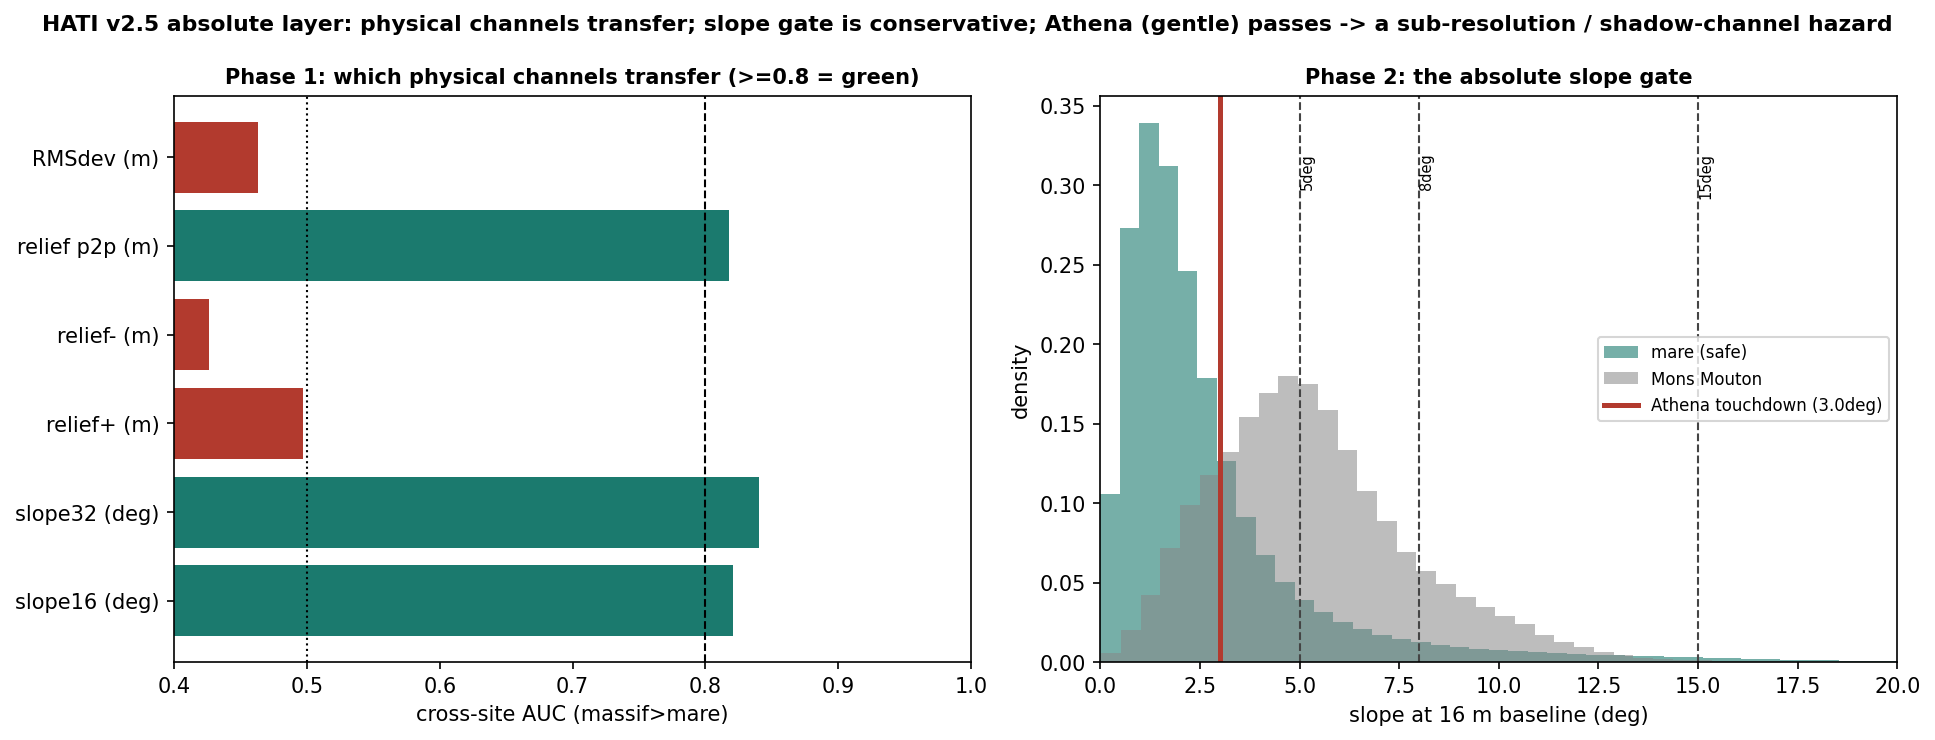
\includegraphics[width=\textwidth]{hati25_absolute_gate.png}
\caption{The absolute layer, on real data. \textbf{Left:} which physical channels transfer
between a smooth mare and the rough massif (green $\ge 0.80$); slope and relief-amplitude
transfer, texture channels do not. \textbf{Right:} the deterministic slope gate, showing the
mare and massif slope distributions on one physical scale, the nominal \ang{8} lander limit,
and the Athena touchdown at \ang{3.0}, which passes.}
\label{fig:gate}
\end{figure}

\begin{figure}[t]
\centering
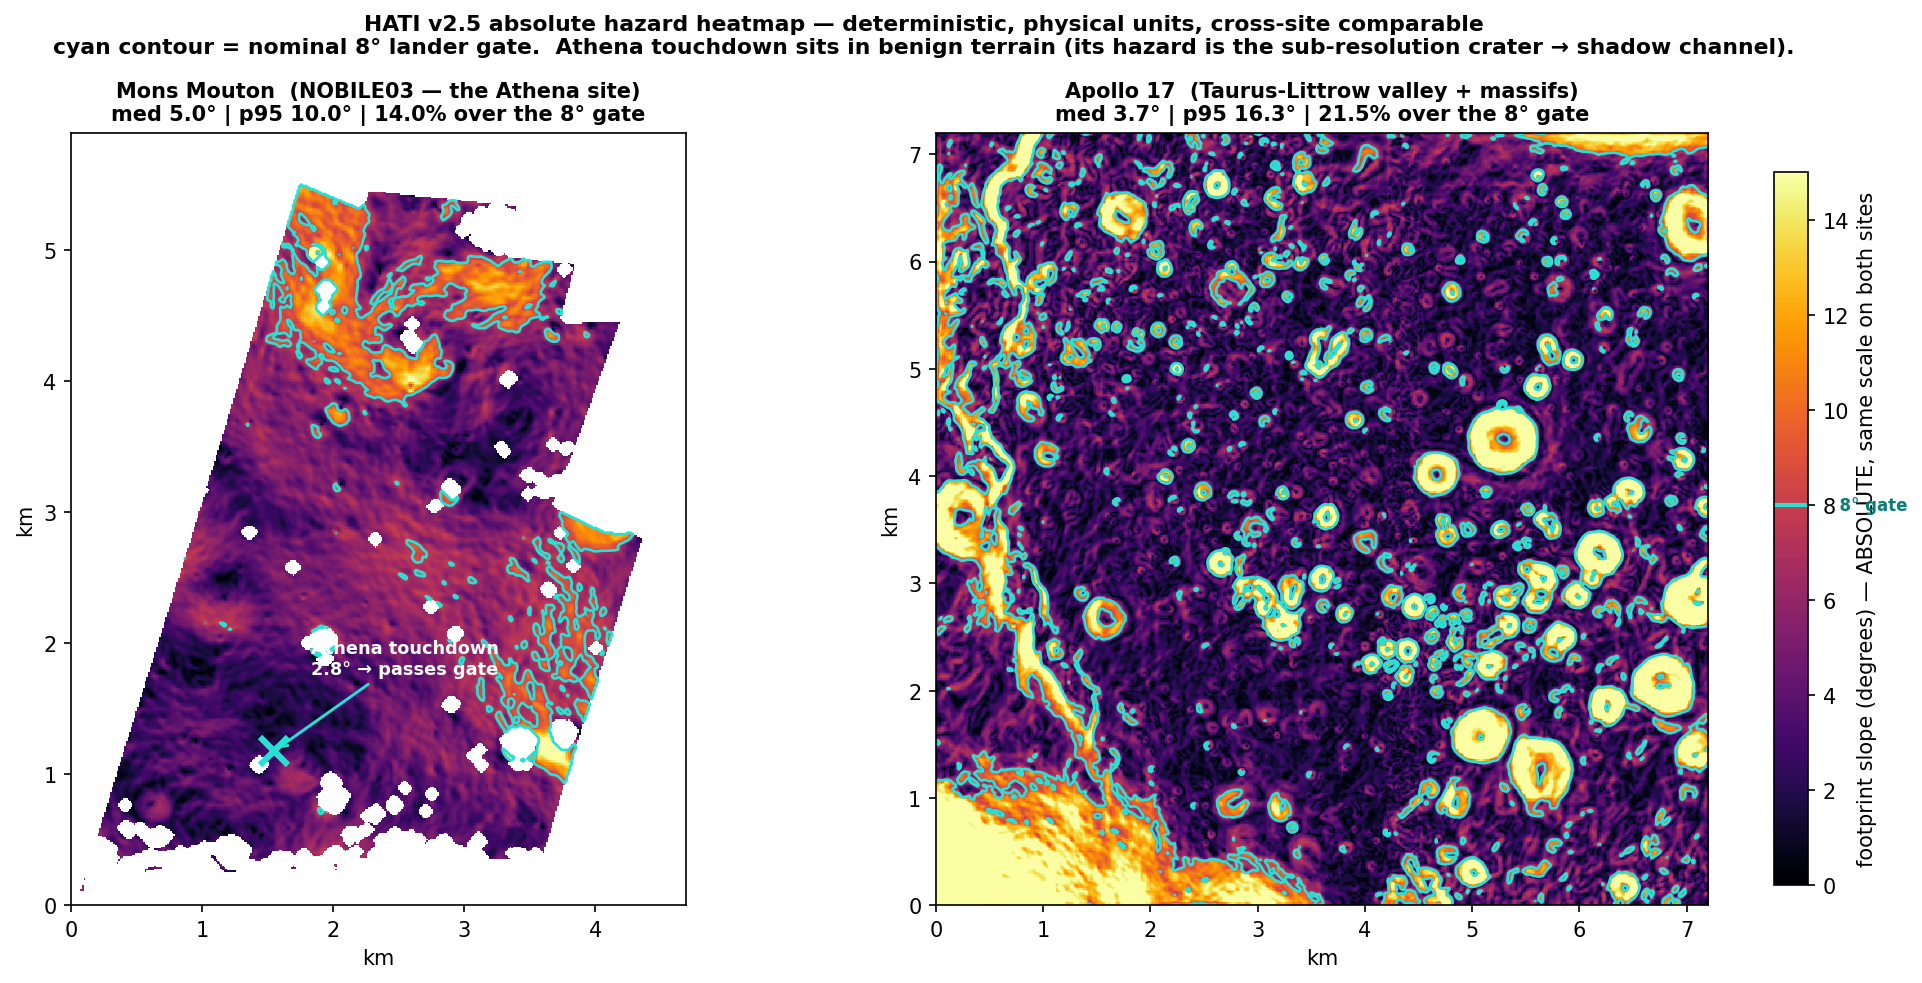
\includegraphics[width=\textwidth]{hati25_heatmaps.png}
\caption{Because the channel is in physical units at matched resolution, two sites are directly
comparable on one colour scale: a \ang{7} slope is \ang{7} on both. Mons Mouton (the Athena
site) with the touchdown marked, beside Apollo\,17's valley and massifs; the cyan contour is the
\ang{8} gate. A per-scene $z$-score heatmap cannot support this comparison.}
\label{fig:maps}
\end{figure}

% =====================================================================
\section{What is established: in simulation only}

\subsection{Shadow kinematics: the sub-resolution channel}
A single shadow photograph cannot tell a real shadow from a dark rock, cannot fix an obstacle's
sign or height without assuming flat ground, and only sees obstacles lit to cast toward the
camera under one Sun. The shadow-kinematics channel removes all three by treating the Sun as a
moving probe over a \emph{solar sweep} (many orthophotos of one site under different solar
azimuths). A true obstacle's shadow pivots about a fixed base while its length tracks the
elevation; a dark albedo mark does not move. Accumulating one vote at the up-Sun base of every
detected shadow makes a real obstacle's votes \emph{converge} (its height falls out of the
length statistics) while an albedo mark's votes \emph{smear} and self-cancel
\autocite{hapke1984,sato2014}.

On a synthetic scene with known truth (\num{70} obstacles of \SIrange{0.3}{3}{\meter} with
sub-resolution footprints, plus \num{40} adversarial albedo and streak decoys, rendered under a
\SIrange{0}{360}{\degree} sweep at \ang{5} elevation), the detector recovers heights to an RMS
error of \SI{0.24}{\meter}, holds detection AUC at \num{0.99}, and drives decoy confidence to
zero while genuine obstacle confidence accumulates (a separation of order \num{8000} at full
sweep; \cref{fig:kin}). We are careful about the claim: the win is on \emph{height, false-alarm
rate and completeness}, not on the detection AUC, which saturates because the orientation gate
alone rejects round decoys in a single frame.

\begin{figure}[t]
\centering
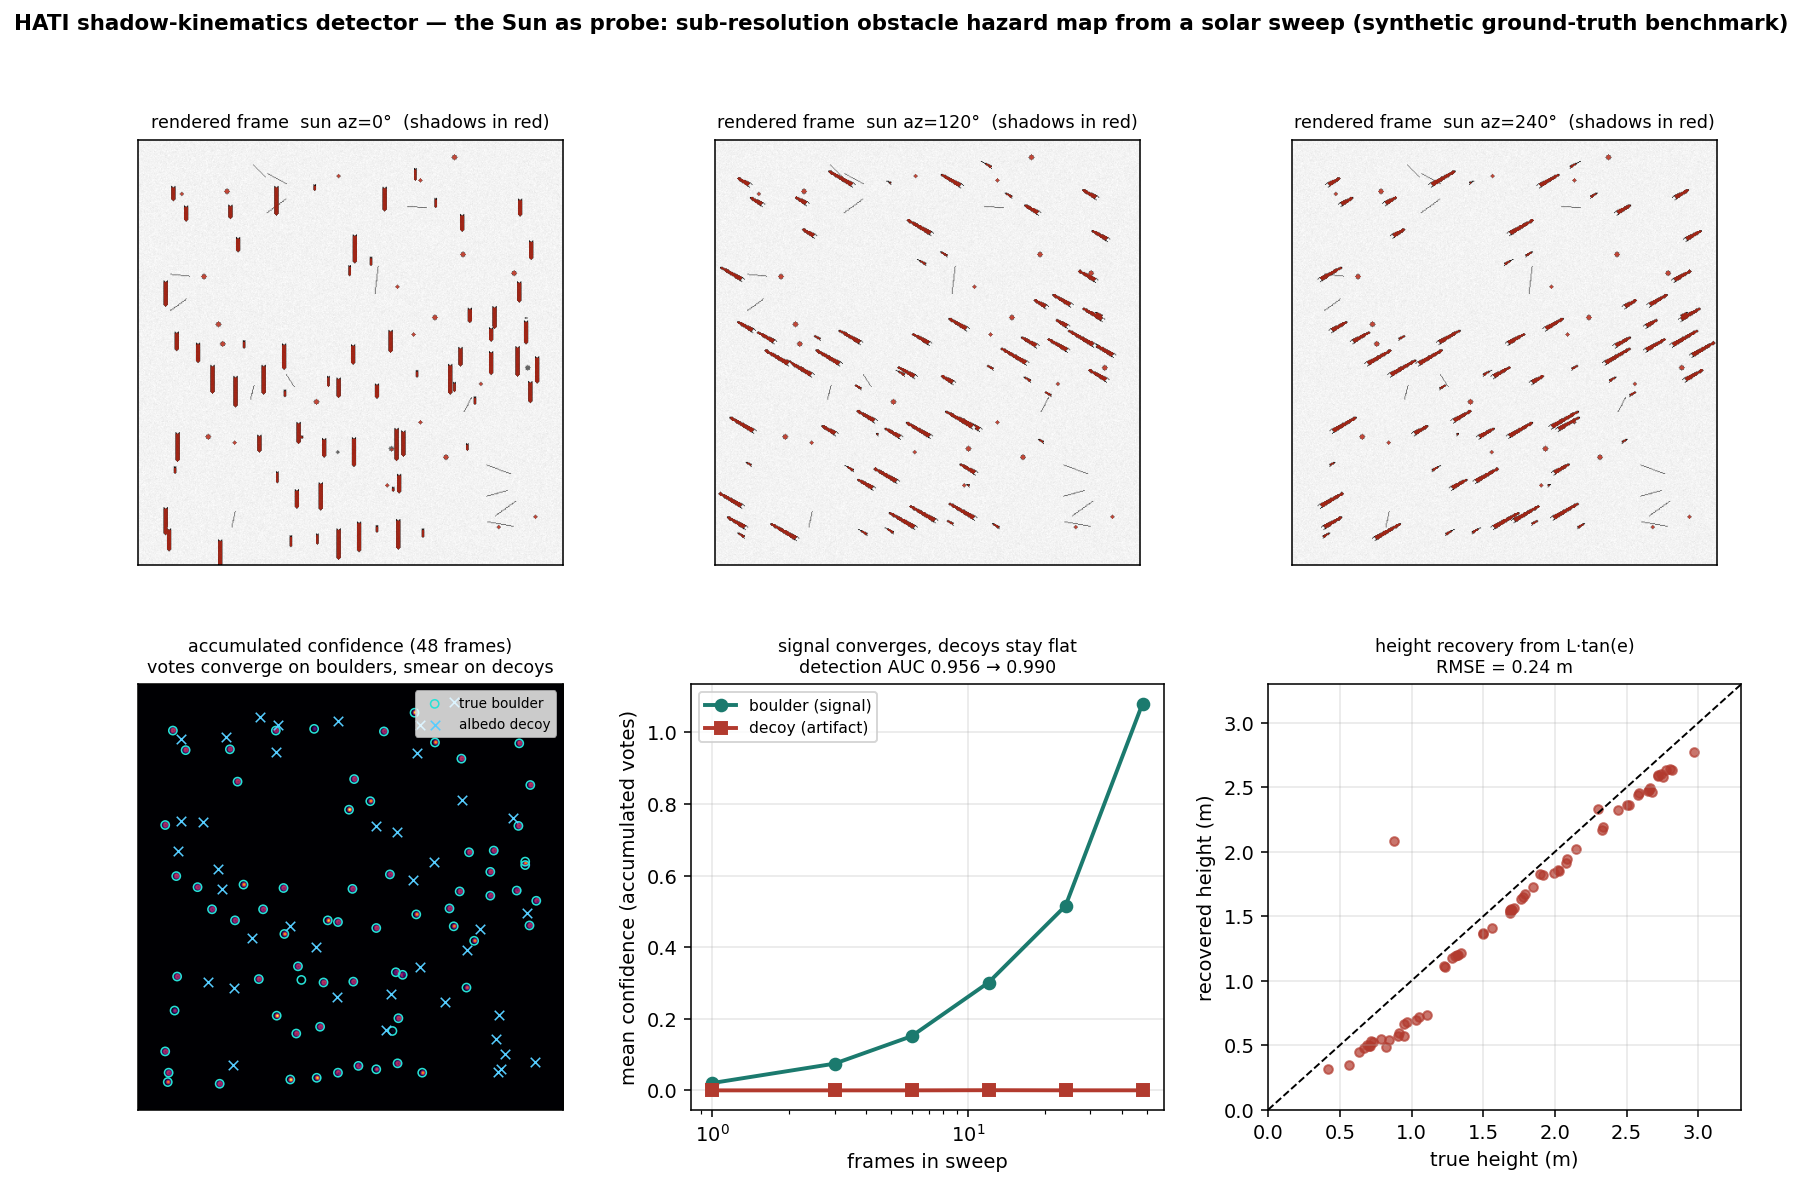
\includegraphics[width=\textwidth]{shadow_kinematics_benchmark.png}
\caption{Shadow kinematics on synthetic ground truth. \textbf{Top:} one scene under solar
azimuths \ang{0}, \ang{120}, \ang{240}, where the shadows (red) pivot about their casters.
\textbf{Lower left:} accumulated confidence after 48 frames converges on the true obstacles
(cyan) and never settles on the decoys (blue). \textbf{Lower middle:} obstacle confidence grows
with sweep size while decoy confidence stays at zero. \textbf{Lower right:} recovered vs true
height, RMS error \SI{0.24}{\meter}.}
\label{fig:kin}
\end{figure}

\subsection{The sweep exists}
The method needs azimuth diversity, so we checked the archive is adequate before committing to
ingestion. A query of the NASA Orbital Data Explorer over the Athena site returns \num{696}
LROC narrow-angle frames, \num{525} with the Sun above the horizon, spanning
\SIrange{2010}{2024}{} and filling all twelve \ang{30} azimuth sectors. The sweep is real and
over-determined; what is missing is the co-registration to turn those frames into a usable
stack.

% =====================================================================
\section{Evidence ledger}

The single most useful thing for a reviewer is an honest map of claim to evidence
(\cref{tab:ledger}). ``Real'' means measured on flight or archival data; ``Synthetic'' means
demonstrated in simulation with known truth; ``Planned'' means designed but not yet run.

\begin{table}[h]
\centering\small
\caption{What is proven, and how.}
\label{tab:ledger}
\renewcommand{\arraystretch}{1.15}
\begin{tabular}{p{8.6cm} c p{3.5cm}}
\toprule
Claim / capability & Evidence & Metric \\
\midrule
Heatmap ranks the Athena touchdown high \emph{within its scene} & Real & $z=3.22$, worst few \% \\
Heatmap is a relative ranker, \emph{not} a calibrated P(loss) & Real (by control) & n/a \\
Shadow census finds sub-resolution obstacles at the site & Real & $\sim$\num{1400}/\si{\kilo\meter\squared} \\
Resolution-ladder recovery (shadow / heatmap) & Real & AUC $0.83$--$0.99$ / $0.86$--$0.93$ \\
Eight texture channels score below chance and were removed & Real (negative) & AUC $0.342$--$0.432$ \\
Physical channels \emph{do} transfer between sites & Real & AUC $0.82$--$0.84$ \\
Absolute slope gate: conservative + specific & Real & mare FA \SI{5.3}{\percent} @ \ang{8} \\
Athena passes the gross-terrain gate (is sub-resolution) & Real & \ang{3.0} slope \\
Shadow kinematics separates obstacles from albedo & Synthetic & decoy conf.\ $\to 0$ \\
Shadow kinematics measures obstacle height & Synthetic & RMSE \SI{0.24}{\meter} \\
An azimuth-diverse sweep exists over the site & Real (archive) & 525 lit frames, 12/12 sectors \\
Real-data shadow-kinematics obstacle map & \textbf{Planned} & n/a \\
Fused, calibrated absolute hazard map & \textbf{Planned} & n/a \\
Site-held-out validation with frozen gates & \textbf{Planned} & n/a \\
\bottomrule
\end{tabular}
\end{table}

% =====================================================================
\section{Forward plan: why and how}

The plan has one milestone that matters and three that package it. We give each a rationale and
a method.

\subsection{Real-data shadow kinematics (the milestone)}
\emph{Why.} Until the kinematics detector runs on a real azimuth-diverse sweep, HATI's central
claim, that it senses the sub-resolution hazards the maps miss, is proven only in simulation.
This is the step that turns a promising estimator into a result on the Moon.
\emph{How.} Build an ingestion pipeline that selects an azimuth-spread subset of the 525 lit
frames, calibrates and map-projects each (ISIS: \texttt{lronac2isis} $\to$ web
\texttt{spiceinit} $\to$ \texttt{lronaccal} $\to$ \texttt{cam2map} to polar stereographic), and
sub-pixel co-registers them to the reference grid. The co-registration error budget is the real
risk: a mislocated shadow base blurs the confidence peak and biases the height, so quantifying
that budget on real frames is the first task, not an afterthought.

\subsection{The integrated absolute hazard map}
\emph{Why.} The gross-terrain gate and the sub-resolution obstacle layer are still separate
scripts; a lander needs one map. \emph{How.} Combine the deterministic slope/relief gate with
the kinematics obstacle density through a threshold-anchored noisy-OR, then calibrate the result
against outcomes so the output is a defensible strike probability of Poisson form,
$P=1-\exp(-\lambda A)$, with $\lambda$ the density of obstacles above the lander's clearance and
$A$ the footprint area, reported honestly as a relative hazard index until enough ground truth
exists to calibrate it into an absolute one.

\subsection{Held-out validation}
\emph{Why.} Every number above is either within-scene or on sites used to reason about the
method. The credible test is generalisation. \emph{How.} Freeze the gates and thresholds, then
run the whole pipeline untouched on a site it has never seen, and report the detection and
false-alarm rates that result. No knob may move after freezing.

\subsection{Capstone and portable core}
\emph{Why.} The work is currently spread across a v2.0 architecture paper, a shadow-kinematics
note, and this report; it needs one honest end-to-end account, and the detection engine needs to
be a clean module rather than a pile of scripts. \emph{How.} Fold the cross-site reorientation,
the absolute gate, the kinematics channel with its real result, and the fused map into a single
v2.5 paper, and factor the detector into a reusable core.

\subsection{Hardening (not blocking)}
A Diviner rock-abundance cross-check of the shadow-derived obstacle density, and an independent
higher-resolution validation, would harden the case but are not required to call the method
established.

\begin{limitbox}
The load-bearing gaps, stated for the reviewer. (1) The sub-resolution channel is unproven on
real imagery; everything about it rests on a synthetic benchmark that is favourable by
construction (flat background, two decoy types). (2) There is no calibrated probability anywhere
in the pipeline yet: the heatmap is a relative ranker and the strike probability is not yet
tied to outcomes. (3) All cross-site numbers involve sites used to develop the method; the
held-out test is not yet done. (4) The shadow height law assumes locally flat ground; real
slopes bias it, and correcting that needs the same multi-illumination stack we have not yet
ingested.
\end{limitbox}

% =====================================================================
\section{Questions we would most like pressed}

We are sending this out precisely to have it challenged. The critiques we would value most:
\begin{itemize}
\item Is the up-Sun-base voting estimator biased in a way the synthetic test hides, for
example on real terrain where shadows fall across slopes rather than flat ground?
\item Is the noisy-OR the right fusion for combining a deterministic gate with a probabilistic
obstacle layer, or does it double-count correlated evidence?
\item Is a resolution ladder on degraded orbital data a fair proxy for real detection
performance, or does anti-aliased degradation flatter the method?
\item What ground truth would make a \emph{calibrated} strike probability defensible, given how
few instrumented lunar landing outcomes exist?
\item Is the cross-site transfer of slope and relief (AUC $\sim0.8$) strong enough to anchor an
absolute gate, or is \num{0.8} simply not good enough for a safety-critical call?
\end{itemize}

\medskip\hrule\medskip
\noindent\footnotesize\textit{Reproducibility.} The channels, controls, gate, sweep query and
kinematics detector are the scripts \texttt{athena\_counterfactual.py},
\texttt{mare\_control\_v2.py}, \texttt{hati25\_absolute\_gate.py}, \texttt{solar\_sweep\_query.py}
and \texttt{shadow\_kinematics.py}; each is deterministic given its stated inputs. Companion
documents: the v2.0 architecture paper and the shadow-kinematics method note.

\printbibliography

\end{document}
